
\subsection{Interpretation of Results}

The ablation results provide direct evidence for the role of auxiliary objectives in shaping the encoder representation. Adding MC dropout to the deterministic Base TCN leaves point-prediction MSE essentially unchanged ($+0.005\%$), confirming that MC dropout's primary contribution is uncertainty estimation rather than forecasting improvement. Activating the dynamic-weight regularizer and the feature-attribution loss together (without AUAA) produces the largest single jump in MSE ($-26.25\%$), demonstrating that the composite objective itself not merely model capacity drives the reduction. Adding AUAA on top of the auxiliary objectives produces near-equivalent MSE ($-25.19\%$): AUAA's contribution is therefore most visible in \emph{anomaly scoring} (uncertainty-gated attention re-weights time steps with high $\sigma_t$) rather than in forecasting metrics that average over time.

The dynamic weight adapter's central tendency $\bar{\alpha} = 0.527$ on the test split sits slightly above $0.5$, indicating mild bias toward reconstruction error in this indoor-air-quality regime. The observed range $\alpha \in [0.003, 0.537]$ confirms that the gating module remains responsive: a small subset of windows triggers near-zero $\alpha$ (uncertainty-dominated scoring) while the dominant operating mode lies near the central tendency. The adapter learns this context dependence end-to-end without manual threshold tuning.

\subsection{Comparison with Prior Stochastic TCN Frameworks}

Our framework extends stochastic TCNs along three architectural dimensions. First, \textbf{uncertainty integration depth}: prior work~\cite{ghimire_electricity_2025, cui_sde-hnn_2025} applies uncertainty post hoc as a scoring term, while our AUAA feeds it into attention computation, consistent with the epistemic/aleatoric decomposition formalized by Kendall and Gal~\cite{kendall2017uncertainties}. Second, \textbf{adaptive vs.\ fixed scoring}: our dynamic weight adapter replaces static $\alpha$ with a context-sensitive mechanism. Third, \textbf{explanatory ambition}: the framework includes a per-sensor attribution head, although our audit (Section~4.7) shows it is not yet causally faithful, so we present it as an exploratory component rather than a delivered capability over prior frameworks~\cite{audibert2020usad, malhotra2016lstmed, zhao2020mtadgat}. The cross-dataset improvement on SKAB ($8.8\times$ F1, $14.4\times$ recall over the Base TCN; \cref{sec:skab_cross_dataset}) confirms that these architectural differences yield measurable gains beyond the IAQ domain. Benchmarked against twelve established detectors under a single unified protocol (\cref{table:skab_baselines}), the proposed model attains the best F1 and the best recall of the panel, while the strongest reconstruction baselines retain higher precision and a marginally higher ROC-AUC. We therefore position the contribution honestly: it is a \emph{recall-oriented} detector whose advantage is the recovery of slow, partial fault signatures that reconstruction-only methods miss, rather than a method that uniformly dominates every metric.

Against the broader families the reviewer raises, the novelty is one of \emph{integration} rather than a new estimator or backbone. Bayesian/stochastic TCNs~\cite{ghimire_electricity_2025, cui_sde-hnn_2025} and uncertainty-aware transformers attach predictive uncertainty as an output-level scoring term; graph-based detectors (MTAD-GAT~\cite{zhao2020mtadgat}) model inter-sensor structure but not reliability; and interpretable industrial monitors add post-hoc explanations. Our framework instead routes the MC-dropout uncertainty \emph{back into} the computation---gating attention (AUAA) and conditioning a learned reconstruction/uncertainty blend (Dynamic Weight Adapter)---and pairs it with a distribution-free operating guarantee. The empirical value of this integration, rather than of the uncertainty estimator itself, is established in two ways above: the deep-ensemble comparison shows the estimator choice is not the source of the gain, and the unified twelve-method benchmark (\cref{table:skab_baselines}) shows the integrated model leads on F1/recall. The positioning of \cref{table:positioning} summarizes which of these four properties---uncertainty quantification, adaptive attention, sensor adaptation, and feature attribution---each family provides.

\subsection{Uncertainty Calibration}

Qualitatively, MC dropout uncertainty estimates tracked prediction difficulty: uncertainty increased during rapid environmental transitions (morning ventilation onset, occupancy changes) and decreased during stable nighttime periods. \cref{fig:uncertainty_calibration} reports the reliability diagram on the test split (left) alongside the distribution of predictive standard deviations (right). The reliability diagram shows that the model's calibrated predictive intervals are mildly \emph{conservative}: empirical coverage sits above the diagonal at low-to-moderate nominal confidence (intervals slightly wider than required) and converges to near-perfect calibration at the high-confidence levels relevant for alarms (empirical coverage $\approx 0.95$ at the $95\%$ nominal level). The raw MC-dropout epistemic standard deviation $\boldsymbol{\sigma}_t$ shown in panel~(b) (mean $\bar{\sigma}=6.18\times 10^{-4}$) is only the epistemic component and is necessarily narrower; the calibrated interval used for the reliability curve combines it with the learned variance head. In either case the distribution-free Chebyshev bound used for threshold selection (Section 3.6) provides the deployment-time FP-rate guarantee independently of this calibration profile. The architectural integration of uncertainty distinguishes this work from standalone calibration studies~\cite{gal2016dropout_bayesian, lakshminarayanan2017ensembles}.

\begin{figure}[H]
\centering
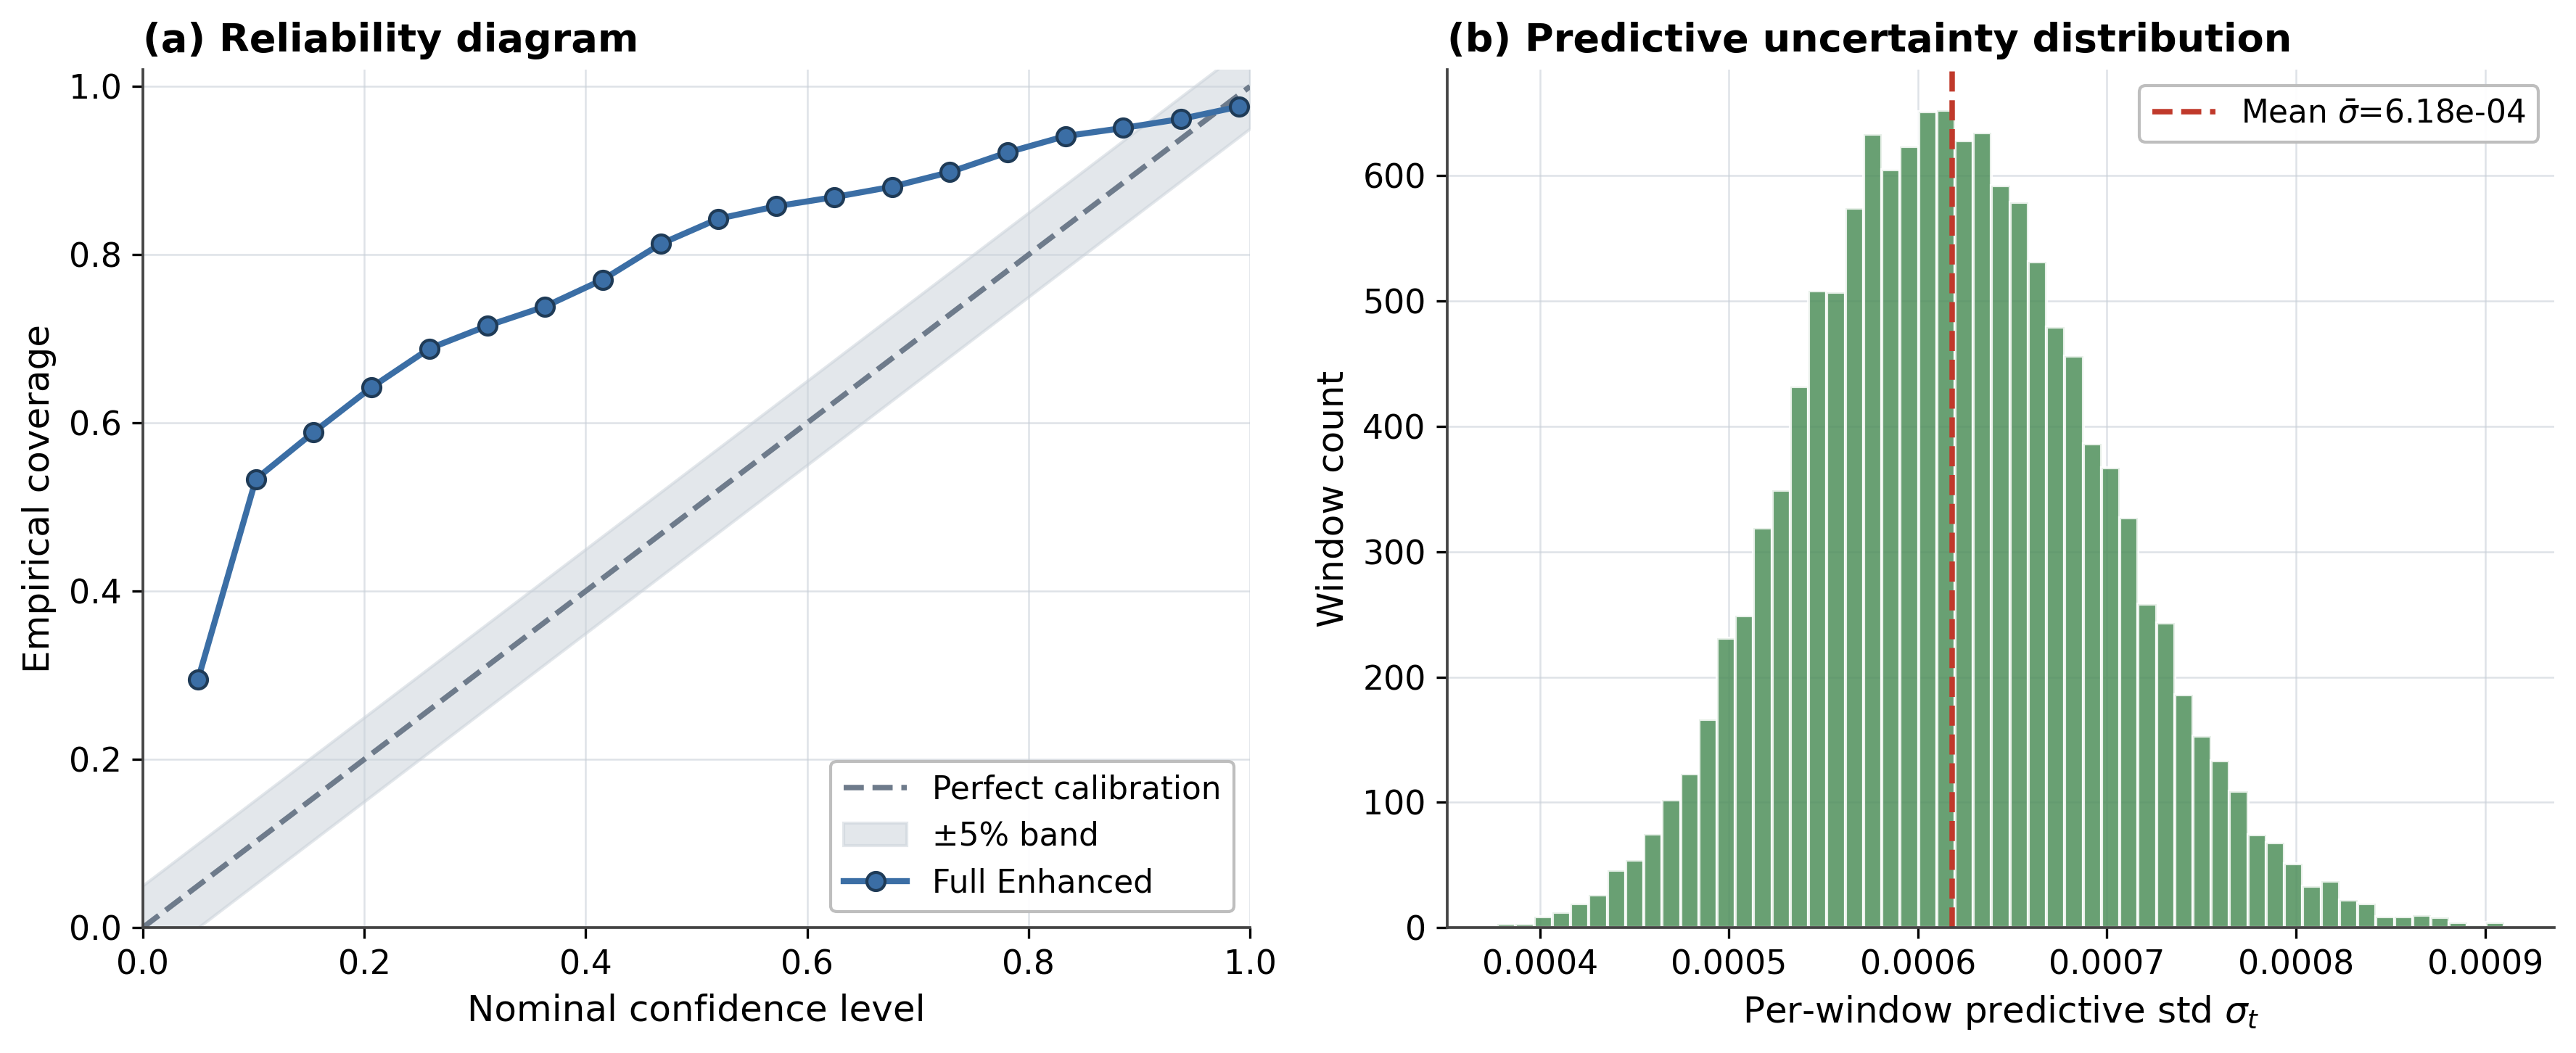
\includegraphics[width=\textwidth]{images/08_uncertainty_calibration.png}
\caption{Uncertainty calibration on the held-out test split. \textbf{(a)} Reliability diagram (empirical coverage vs.\ nominal confidence; the diagonal is perfect calibration, below it is over-confidence). \textbf{(b)} Histogram of per-window predictive standard deviation $\boldsymbol{\sigma}_t$ ($M=50$), centred at $\bar{\sigma} = 6.18\times 10^{-4}$.}
\label{fig:uncertainty_calibration}
\end{figure}

\subsection{Sensor-Specific Design Justification}

Each architectural choice is motivated by a concrete sensor-characteristic argument:

\textbf{AUAA justified by sensor heterogeneity.} The uncertainty gate $1/(1 + \sigma_t)$ is motivated by the observation that sensor noise variance varies both across sensor types (e.g., electrochemical VOC vs.~thermistor temperature) and over time (sensor aging, environmental interference). A mechanism that uniformly treats all attention positions is suboptimal when some positions carry substantially more reliable information than others.

\textbf{Dynamic weighting justified by sensor degradation.} Fixed-weight scoring implicitly assumes constant sensor quality—an assumption violated by real sensor deployments where CO\textsubscript{2} sensor drift and VOC sensitivity degradation evolve on timescales of days to weeks. The dynamic adapter's GRU state provides memory of recent sensor behavior, enabling adaptation to degradation trends.

\textbf{Attribution justified by maintenance workflows.} In facility management, an anomaly attributed to CO\textsubscript{2} triggers HVAC inspection, while one attributed to dust triggers filter replacement—different sensor attributions lead to different operational responses. The attribution head is intended to provide this sensor-level granularity; we include it for this reason but, per the faithfulness audit (Section~4.7), it does not yet do so reliably and is reported as a limitation rather than a solved capability.

\subsection{Design Extensions and Deployment Considerations}

The sensor-specific design principles established in this work suggest natural extensions. Training under normal-operation assumptions means contamination by undetected anomalies can bias predictive distributions, robust training strategies such as trimmed loss functions offer a direct mitigation path. The current single-step prediction scope can be extended to multi-horizon forecasting using long-context Transformer variants such as Informer~\cite{zhou2021informer} or TimesNet~\cite{wu2022timesnet} for detecting gradual drift patterns that emerge over longer timescales. Graph-attention extensions such as MTAD-GAT~\cite{zhao2020mtadgat} provide a path for modelling explicit inter-sensor dependencies that the current channel-independent architecture does not capture. For higher-frequency sensor streams (e.g., 100~Hz vibration monitoring), model distillation or reducing the number of MC samples allows architectural benefits to be preserved within tighter latency constraints. Assumptions regarding a fixed sensor set can be relaxed through dynamic input filtering, and online learning variants can address conceptual shifts in non-stationary environments.

\subsection{Limitations}

We state the boundaries of the present study explicitly. \textbf{(i) Attribution faithfulness.} The feature-importance head is not yet causally faithful: under a controlled $+6\sigma$ single-channel spike its top-ranked channel matches the perturbed one only $12.7\%$ of the time (chance $12.5\%$) and it collapses onto a single channel, so we report it as an architectural placeholder and a future-work target rather than a validated explanation (Section~4.7). \textbf{(ii) Effect size.} The IAQ forecasting gain, while statistically significant (Section~4.3), is modest in absolute MSE; we have accordingly reframed the contribution around detection recall and operational guarantees rather than headline accuracy, and we avoid claiming large forecasting improvements. \textbf{(iii) Component interactions.} The ablation (\cref{table:ablation}) varies components cumulatively and shows no negative interaction, but it is not a full $2^3$ factorial, so synergy versus independence among AUAA, the dynamic adapter, and the attribution head is only partially resolved. \textbf{(iv) Domain coverage.} Both evaluation domains (indoor air quality and industrial water circulation) are comparatively stationary; generalization to highly non-stationary or heterogeneous cyber-physical streams, and robustness to adversarial perturbations and inter-sensor synchronization errors (beyond the channel-masking and Gaussian-noise tests of Section~4.8), remain open. \textbf{(v) Theoretical scope.} The Monte-Carlo convergence result (\cref{thm:mc_convergence}) is a standard SLLN/CLT consequence repurposed here to justify the sample budget $M$ rather than a new probabilistic result; its role is to make the $O(M^{-1/2})$ trade-off explicit, and the Chebyshev bound, though valid and empirically respected (\cref{table:chebyshev_calib}), is intentionally conservative for near-Gaussian scores.